\chapter{Modellierung}
In diesem Kapitel sollen die Anforderungen aus den Interviews praktisch erhoben werden, die Referenzarchitekturen erstellt werden und die konstruierten Referenzarchitekturen folgend auch verglichen werden.
\section{Anforderungserhebung}
Wie in \autoref{theorie:referenzmodellierung} beschrieben, müssen Referenzmodelle einen subjektiven Empfehlungscharakter besitzen, damit sie akzeptiert und wiederverwendet werden. Dafür muss ein Abgleich mit den Anforderungen der Nutzenden geschehen. Um dies zu erreichen, wurden im Anhang transkribierte Interviews (vgl. \anhangref{anhang:interview-philipp-22.03.2021}, \anhangref{anhang:interview-peter-24.03.2021}, \anhangref{anhang:interview-ralph-24.03.2021}) durchgeführt. Daraus ergibt sich das in \autoref{abb:TopLevelEchtzeitRA} gezeigte Diagramm, welches die Anforderungen der individuellen Stakeholder an Dekompositionstiefe, Anwendbarkeit und Allgemeingültigkeit darstellt.

\begin{figure}[H]
\centering
\spideroverview
%{P. Arnold}
{5}{3}{3}
%{R. Briegel}
{3}{3}{1}
%{P. Erbacher}
{2}{4}{5}
\caption{Ergebnisse der Interviews}
\label{abb:DimensionenUebersicht}
\end{figure}
Durch die Interviews liessen sich folgende Durchschnitte errechnen: Dekompositionstiefe wurde im Schnitt mit $3,\overline{3}$ bewertet. Die Anwendbarkeit wurde ebenfalls mit $3,\overline{3}$ bewertet. Die Allgemeingültigkeit hingegen hat nur einen Schnitt von $3$. Entsprechend sollten Dekompositionstiefe und Anwendbarkeit priorisiert werden, während die Referenzarchitektur organisationsspezifischer sein darf. 
In den folgenden Referenzarchitekturen wird in mehrere Dekompositionen unterteilt. In der Datenverarbeitungssequenz werden mit Hilfe eines Sequenzdiagramms die Abläufe zur Datenverarbeitung mit dem zu betrachtenden Dienst, ausgehend von \AWSIOT{} Core als Messagebroker gezeigt.
Die Verteilungssicht soll sowohl die Interaktion der Dienste untereinander, als auch grob das durchzuführende Deployment zeigen. Die Bausteinsicht zeigt wichtige Elemente der einzelnen Dienste auf, die konkret untereinander interagieren. So ist die konkrete Untereinheit, die Daten von \AWSIOT{} Core an andere Dienste versendet eine \AWSIOT{} Core Rule, welche aufzuzeigen wäre. \TodoW{Genauere Auswirkungen}

Für die Operations wird vorausgesetzt, dass der \ac{AWS}-native Dienst CloudWatch zur Überwachung eingesetzt wird. 
\begin{figure}[H]
\centering
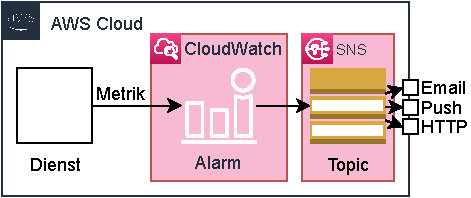
\includegraphics[width=0.66\textwidth]{graphics/CloudWatch-Monitoring}
\caption{CloudWatch Monitoring}
\label{abb:CloudWatchMonitoring}
\end{figure}
CloudWatch erfasst zentralisiert Metriken aller Dienste und löst bei nutzerdefinierten Überschreitungen einen Alarm aus, welcher dann via \ac{SNS} versendet werden kann (siehe \autoref{abb:CloudWatchMonitoring}). Dabei kann bei Metriken mit hoher Varianz die Cloudwatch eigene Anomalienerkennung verwendet werden oder die Schwellwerterkennung.



Zusätzlich haben sich folgende Anforderungen ergeben:
\begin{itemize}
\item Anwendbarkeit auf Monitoringdaten (IT) (\anhangref{anhang:interview-philipp-22.03.2021}, \anhangref{anhang:interview-peter-24.03.2021})
\item Anwendbarkeit auf Sensordaten (\ac{IoT}) (\anhangref{anhang:interview-philipp-22.03.2021}, \anhangref{anhang:interview-peter-24.03.2021}, \anhangref{anhang:interview-ralph-24.03.2021})
\item Wertschöpfung für das Unternehmen wichtig
\item akzeptabel und problemlösend für Domäne
\item Handling von Events, Messwerten und \enquote{Streaming} (\anhangref{anhang:interview-peter-24.03.2021})
\end{itemize}

% \begin{figure}[H]
% \centering
% 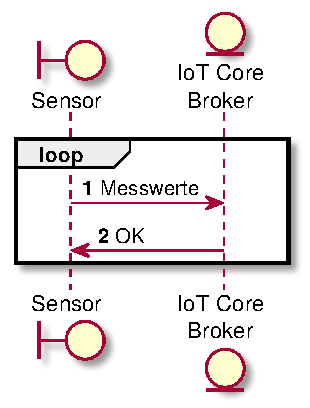
\includegraphics[height=0.3\textheight]{graphics/dateneinspeisung.pdf}
% \caption{Sequenzdiagramm Dateneinspeisung}
% \label{abb:SequenceEinspeisung}
% \end{figure}

Im Folgenden werden die Referenzarchitekturen entworfen und miteinander verglichen, um mögliche Stärken und Einsatzgebiete zu identifizieren.

\section{Echtzeitverarbeitung}\label{chap:ra-rt}
Aufgrund des in \autoref{tab:bewertungsmatrix-echtzeit} durchgeführten Vergleiches, den Kinesis (Data Streams und Analytics) anführte, wird im Folgenden die Referenzarchitektur für die Echtzeitverarbeitung mit Kinesis Data Streams und Analytics entworfen. Diese Referenzarchitektur entspricht dem in \autoref{chap:bestehende_ras} vorgestellten Konzept einer $\kappa$-Architektur.

\subsection{Datenverarbeitungssequenz}
In \autoref{abb:SequenceEchtzeitRA} wird die durchlaufene Sequenz für eingehende Daten gezeigt. Nach initialer Übertragung via \ac{MQTT} an \AWSIOT{} Core, folgt die Übertragung in Kinesis Data Streams, welche die Daten gepuffert an Kinesis Data Analytics sendet. 

\begin{figure}[H]
\centering
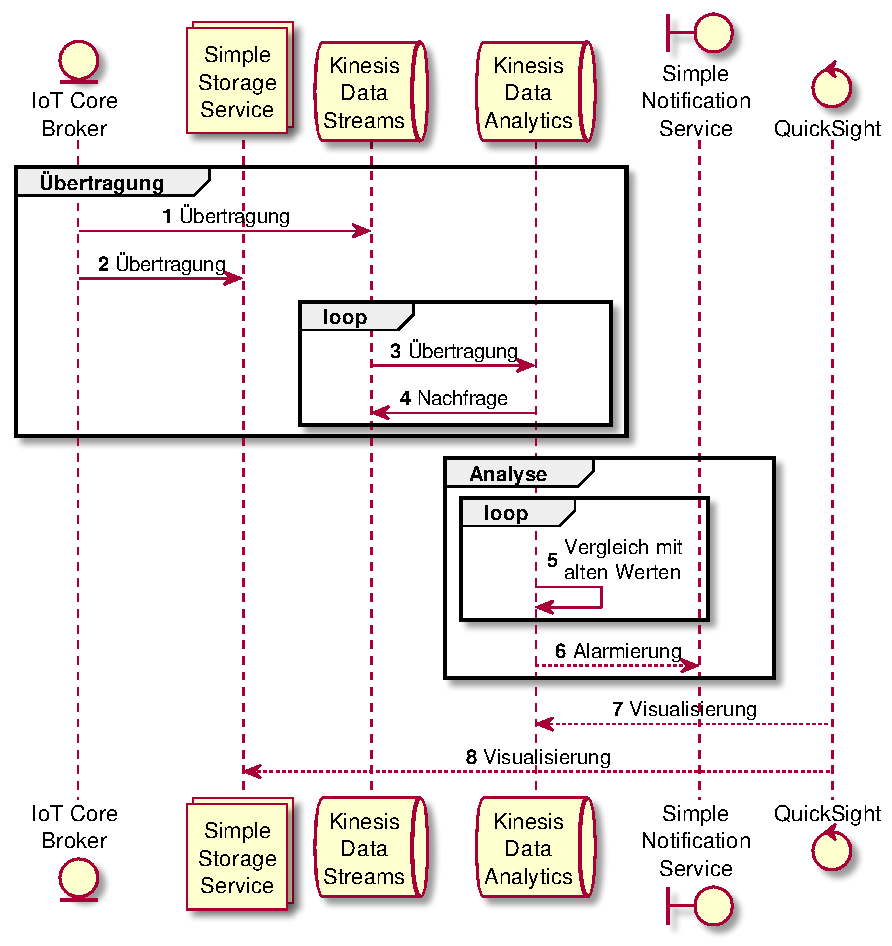
\includegraphics[height=0.6\textheight]{graphics/echtzeit-ra.pdf}
\caption{Sequenzdiagramm Echtzeitreferenzarchitektur}
\label{abb:SequenceEchtzeitRA}
\end{figure}

\subsection{Verteilungssicht}
Folgend ist die Verteilungssicht der Echtzeitreferenzarchitektur gezeigt. Gemeinsame Variationspunkte dieser und folgender Dekompositionen bekommen den Buchstaben G und eine fortlaufende Nummer und werden nur einmal erklärt.
\begin{figure}[H]
\centering
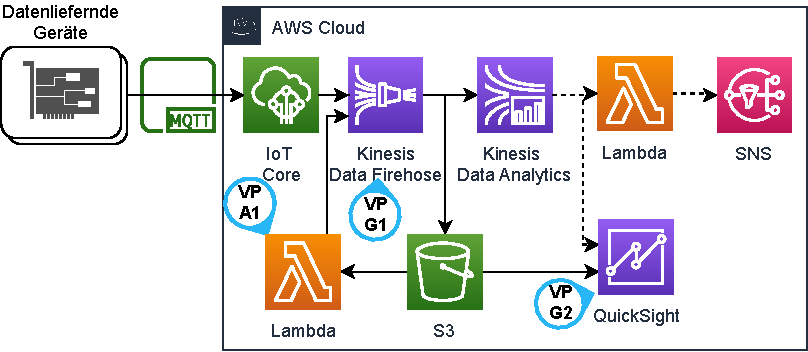
\includegraphics[width=\textwidth]{graphics/Echtzeit-RA-Overview-Firehose}
\caption{Verteilungssicht mit Data Firehose}
\label{abb:TopLevelEchtzeitRA}
\end{figure}

\vp{G1}: Je nach Anforderung kann Kinesis Data Firehose oder Kinesis Data Streams verwendet werden. Während die höhere Abstraktion und das einfachere Abrechnungsmodell von Kinesis Data Firehose einen reduzierten Wartungsaufwand hat, bietet Kinesis Data Streams mehr Kontrolle über unterliegende Faktoren wie Datenaufbewahrung und Durchsatz. Kinesis Data Firehose benötigt zwingend ein \enquote{Delivery ziel}. Dies kann beispielsweise ein \ac{S3}-Bucket, eine Redshift Datenbank oder eine Elasticsearch Datenbank sein. In diesem Fall wurde aus Kosten- und Umsetzungserwägungen ein \ac{S3}-Bucket gewählt.



\vp{G2}: QuickSight als \ac{AWS} native Dashboardlösung ist gut geeignet, um schnell Übersicht in Datenanalysen aus Kinesis Data Analytics zu bekommen. Alternativ können auch andere Visualisierungslösungen wie Tableau eingesetzt werden, welche gegebenenfalls jedoch keinen (vollen) Zugriff auf Kinesis Data Analytics haben. Ein weiterer managed Service, den \ac{AWS} für Dashboards anbietet, ist der Amazon Managed Service for Grafana, welcher das Open Source Visualisierungstool Grafana mit den \ac{AWS} eigenen Metriken integriert.\footcite[Vgl.][]{Dutt.2020} In diesem Fall kann der \ac{S3} Bucket verwendet werden, um Dashboards über die Rohdaten zu erstellen. 

\vp{A1}: Sollte es nicht gewünscht sein, Daten erneut in Kinesis Data Firehose einzuspielen, kann auf die Lambdafunktion verzichtet werden. Diese liest, wenn manuell aktiviert, den \ac{S3}-Speicher ein und spielt die erfassten Nachrichten erneut in der selben Sequenz in Kinesis Data Firehose ein. Notwendig wird diese Lambda, wenn historische Daten mit abweichender Analyselogik analysiert werden sollen.

Im Folgenden wird die Verteilungssicht im zweiten Fall von \vpref{G1}, der Verwendung von Kinesis Data Streams gezeigt. Die Auswahl von Kinesis Data Streams ist insbesondere angezeigt, wenn die Nachrichten direkt aufbewahrt werden sollen und direkter Einfluss auf die Performance erwünscht ist.

\begin{figure}[H]
\centering
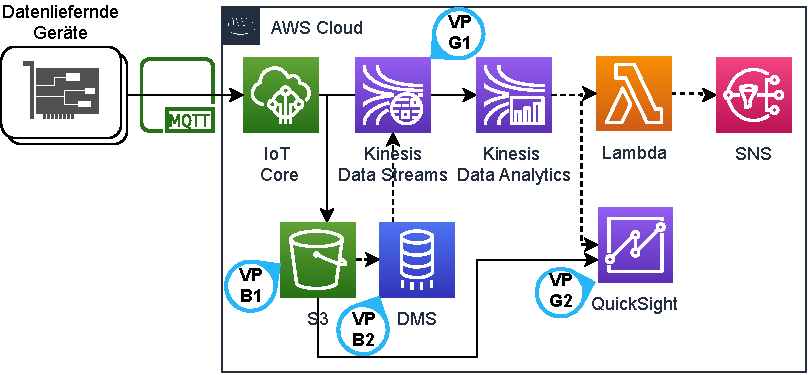
\includegraphics[width=\textwidth]{graphics/Echtzeit-RA-Overview.pdf}
\caption{Verteilungssicht mit Data Streams}
\label{abb:TopLevelEchtzeitRAStreams}
\end{figure}

\textbf{Variationspunkte G1, G2}: Siehe oben: \vpref{G1}, \vpref{G2}

\vp{B1}: Rohdaten in \ac{S3} zu speichern kann Sinn machen, um die Daten später noch einmal analysieren zu können. Nimmt man aber die Theorie der Datenhalbwertszeit zur Hilfe, macht es vielleicht Sinn die Daten statdessen maximal 48h in Kinesis Data Streams zwischenzuspeichern und auf \ac{S3} zu verzichten. Mittels der erweiterten Aufbewahrung $\lbrack$\textit{Data Retention}$\rbrack$ können Analysen mehrfach im Fehlerfall angefordert werden. Da die Preise nach sieben Tagen Aufbewahrung ansteigen und für Aufbewahrung und Abruf doppelt abgerechnet wird, ist zu empfehlen, nach sieben Tagen die Daten zu verwerfen.\footcite[Vgl.][]{AmazonWebServicesInc..o.J.l} Dieser Variationspunkt ist abhängig vom \vpref{G1}, da Kinesis Data Firehose keine erweiterte Aufbewahrung unterstützt und die Daten in \ac{S3} abgelegt werden müssen.

\vp{B2}: \ac{DMS} ist in diesem Szenario dafür gedacht, einmal abgelegte Daten in S3 wieder in Kinesis Data Streams einspielen zu können. Je nach Szenario ist dies, wie bei \vpref{B1} schon erläutert, nicht notwendig.

\subsection{Bausteinsicht}
Unter Berücksichtigung von \vpref{G1} gibt es zwei Bausteinsichten. Dies ist bedingt durch die sich ergebenden architekturellen Änderungen, beim Einsatz von Kinesis Data Streams oder Kinesis Data Firehose. 

\begin{figure}[H]
\centering
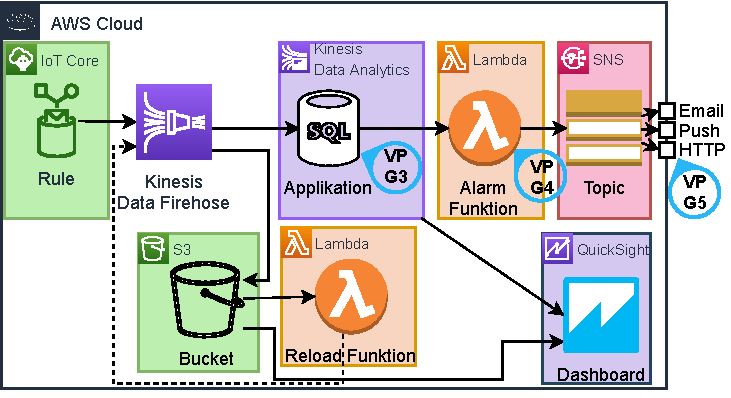
\includegraphics[width=\textwidth]{graphics/Echtzeit-RA-Elements-Firehose.pdf}
\caption{Bausteinsicht mit Data Firehose}
\label{abb:ElementeEchtzeitRA}
\end{figure}

\vp{G3}: Der \ac{SQL} Programmcode, der in Kinesis Data Analytics läuft ist anzupassen. So sind Verarbeitungsfenster, Attributsnamen und aufgerufene Funktionen nach Anforderung zu ändern. Andernfalls kann auch die Funktionalität zur Ausführung eigenen Codes via Apache Flink in Kinesis Data Analytics genutzt werden (dies erlaubt Ausführung von Java, Scala, Python). Dies ist angezeigt, wenn der \ac{SQL}-Dialekt die gewünschten Auswertungen nicht unterstützt, oder eine eigene Implementierung vorgesehen ist.

\vp{G4}: Aufgrund der Notwendigkeit einer Lambda Funktion, um Alarme zu versenden, kann der Code selbst gestaltet werden. Wichtig ist dabei, dass Kinesis Data Analytics die Zustellung von Datensätzen wiederholt, wenn die Lambdafunktion als Rückgabewert ein Array mit den Ids und dem Status wie folgt zurückgibt: \mintinline[breaklines]{json}{[{"recordId": "<ID>", "result": "DeliveryFailed"}]}.\footcite[Vgl.][]{AmazonWebServicesInc..o.J.ay} Die übermittelten Alarme lassen dabei Möglichkeit zur Anpassung. So kann neben dem Titel der Nachricht auch der eigentliche Inhalt angepasst werden. Beispielhaft ist in \anhangref{anhang:echtzeit-codesample} gezeigt, wie eine in JavaScript geschriebene Lambdafunktion aussehen könnte, die via Kinesis Data Analytics angesteuert wird. Diese Funktion gibt selbstständig fehlerhafte Nachrichten zur Wiederverarbeitung an Kinesis Data Analytics zurück, versendet \ac{SNS} Alarme und kann via \ac{MQTT} eine Shutdown Nachricht an das Gerät übermitteln.

\vp{G5}: \ac{SNS} unterstützt mehrere Protokolle für die Übermittlung von Nachrichten. Es können HTTP Webhooks genauso wie mobile Pushbenachrichtigungen oder auch Emails versendet werden. Welches Protokoll mit welchem Verteiler zu wählen ist, muss im \ac{SNS} Topic eingestellt werden. Innerhalb der Cloud Native Solution der SPIRIT/21 hat sich bewährt, den Versand via Email zu nutzen und als Ziel den Email-Verteiler eines Monitoring Teams innerhalb des Tools Microsoft Teams einzustellen. Microsoft Teams zeigt eingegangene Emails an den Emailverteiler dann als Chatnachricht innerhalb des Teams an und benachrichtigt alle Teilnehmenden.

\begin{figure}[H]
\centering
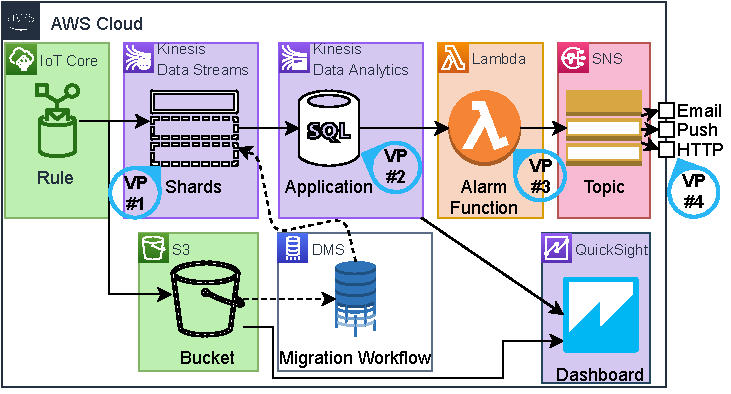
\includegraphics[width=\textwidth]{graphics/Echtzeit-RA-Elements.pdf}
\caption{Bausteinsicht mit Data Streams}
\label{abb:ElementeEchtzeitRAStreams}
\end{figure}
\textbf{Variationspunkte G3, G4, G5}: Siehe oben: \vpref{G3}, \vpref{G4}, \vpref{G5}

\vp{C1}: Die Anzahl an Shards ist essentiell für die Performance von Kinesis Data Streams. Für Workloads mit einem vorhersehbaren Workload ist Anzahl an Shards nach einem Preis/Leistungs Optimum zu ermitteln und zu konfigurieren. Wenn der Workload nicht vorhersehbar ist oder schnell skalieren können soll, sind Alarme im AWS eigenen Monitoring Tool CloudWatch zu erstellen. Im Beispielusecase für die Kostenschätzung ist ein einziger Shard (1MiB/Sekunde, 1000 Nachrichten eingehend) ausreichend. Dies ist bedingt, da Nachrichten mit einer Größe von 1KB, also ca. 1KiB geschrieben werden, bei einem Maximum von 200 pro Sekunde und einem Konsumenten. Es ist besonders auf die \enquote{WriteProvisionedThroughputExceeded} Metrik zu achten, welche bei höheren Werten anzeigt, dass das Hinzufügen von zusätzlichen Shards angebracht wäre. Ebenfalls ist die Metrik \enquote{Incoming Records} zu beachten. Verändert diese sich, deutet das auf einen Fehler im vorgelagerten \AWSIOT{} Core oder in einem Teil der Datenlieferanten hin.

\subsection{Anforderungen}
\begin{itemize}
\item Anwendbarkeit auf Monitoringdaten (IT)\\
Kinesis als System ist gut auf diverse Zeitseriendaten anwendbar. Problematisch ist das eigene Übertragungsformat, welches von Datenproduzenten verlangt, spezielle Schnittstellen zu implementieren. Der von \ac{AWS} vorgesehene Weg, die Kinesis Producer Library ist in Java geschrieben und bindet eine ausführbare C++ Datei ein.\footcite[Vgl.][]{AmazonWebServicesInc..o.J.bg} Im Einsatz mit Monitoringdaten würde dies erfordern, dass die Daten in einem Standardformat aggregiert und dann mittels eines in Java geschriebenen Programms transformiert werden müsste. 
% Alternativ können noch die \enquote{Kinesis Record Aggregation \& Deaggregation Modules for AWS Lambda} von \ac{AWS} verwendet werden, welche die Daten in das aggregierte, kinesiseigene Format umwandeln.\footnote{Siehe \url{https://github.com/awslabs/kinesis-aggregation}} Diese Module haben Sprachkompatibilität zu Java, JavaScript/Node.js und Python.
CloudWatch bietet genau diese Funktionalität mittels der CloudWatch Metric Streams und der CloudWatch Log Subscriptions an.\footcite[Vgl. auch im Folgenden][]{Barr.2021} Bei Metric Streams werden Metriken auf Wunsch in das OpenTelemetry oder das \ac{JSON} Format konvertiert und dann an Kinesis Data Firehose zur Weiterverarbeitung übermittelt. Dabei werden aber nur Metriken erfasst, die einen Zeitstempel jünger als zwei Stunden haben, was manche Metriken, die einmal am Tag versendet werden ausschließt. Zusätzlich muss ein Metric Stream in jeder Region angelegt werden, wo CloudWatch Logs anfallen, was eine Herausforderung in stark verteilten \ac{AWS}-Accounts darstellen kann. Metric Streams kosten 0,003\$ pro 1000 verarbeitete Metriken und zusätzlich die entsprechend anfallenden Data Firehose Gebühren. CloudWatch Log Subscriptions bietet sowohl das Streamen an Kinesis Data Streams, als auch an Kinesis Data Firehose an.\footcite[Vgl. auch im Folgenden][]{AmazonWebServicesInc..o.J.bk} Für jede Loggruppe, die einem Dienst oder einer einzelnen Ressource, wie beispielsweise einer Lambdafunktion zugeordnet sein kann, ist eine Subscription zu erstellen. Um dies zu erleichtern, sollte von Infrastructure as Code Gebrauch gemacht werden, um die Subscription automatisch für jede erstellte Loggruppe einzurichten. Es können benutzerdefinierte Filter eingerichtet werden, um nur relevante Logs zu übermitteln.

Insgesamt scheint die Kinesis Dienstfamilie gut geeignet, um sowohl Logs als besondere Zeitreihendaten, als auch Metriken skalierbar zu verarbeiten.

\item Anwendbarkeit auf Sensordaten (\ac{IoT})\\
Kinesis ist generalisiert ausgelegt, durch die Integration mit \AWSIOT{} Core wird jedoch die Verarbeitung von \ac{IoT} Daten leicht gemacht. 

\item Handling von Events, Messwerten und \enquote{Streaming}\\
Da die Verarbeitungslogik in Kinesis Data Analytics selbst zu schreiben ist, ist die unterschiedliche Behandlung von Events, niedrigfrequenten Messwerten und Streaming implementierungsabhängig. Dabei wäre es zu empfehlen ein Attribut in die übermittelten Nachrichten einzufügen, welches den geanauen Typ der Nachricht definiert und entsprechende Verarbeitungslogiken vereinfacht. Zu diesem Zweck soll das Attribut \mintinline[breaklines]{json}{{"messageType": "<string>"}} dienen. Für Events, die Definitionsgemäß keinen Messwert beinhalten, ist das Attribut mit dem Wert \mintinline[breaklines]{json}{{"messageType": "event"}} zu belegen. Messwerte sollen \mintinline[breaklines]{json}{{"messageType": "meas_low_freq"}} als Wert verwenden. Für hochfrequentes Streaming ist \mintinline[breaklines]{json}{{"messageType": "meas_high_freq"}} zu verwenden.

\item automatisierte operative Entscheidungen\\
Automatisierte Entscheidungen bzw. Handlungen sind mit Kinesis Data Analytics möglich. So könnte die selbe Lambdafunktion, die für die Alarmierung benutzt wird, auch Aktionen auslösen. Vorstellbar wäre, dass die Lambdafunktion über \ac{MQTT} Aktoren ansteuert, weitere Akteure informiert (z.B. die Werksfeuerwehr) oder selbstständig Anweisungen auslöst, die den Alarm beheben (so könnte bei niedrigem Batteriestand eine neue Batterie für einen Sensor geordert werden). 
\end{itemize}


\subsection{Operations} \label{chap:echtzeit_ops}
In \autoref{tab:cloudwatch-metrics-rt} sind die zu überwachenden Metriken von Kinesis Data Streams, \ac{SNS}, \AWSIOT{} Core, Kinesis Data Analytics und Kinesis Data Firehose gezeigt.\footcite[Vgl.][]{AmazonWebServicesInc..o.J.bb}\nzitat\footcite[Vgl.][]{AmazonWebServicesInc..o.J.bc}\nzitat\footcite[Vgl.][]{AmazonWebServicesInc..o.J.az}\nzitat\footcite[Vgl.][]{AmazonWebServicesInc..o.J.ay}\nzitat\footcite[Vgl.][]{AmazonWebServicesInc..o.J.bj}

\begin{table}[H]
\centering
\begin{tabular}{|l|l|l|l|}
\hline
Dienst & Metrik & Ursache & Detektionsart \\ \hline
\rowcolor[HTML]{F5F5F5} 
\ac{SNS} & NumberOfNotificationsFailed & Dienstfehler & Schwellwert \\ \hline
 & RuleMessageThrottled & Dienstfehler & Schwellwert \\ \cline{2-4} 
\multirow{-2}{*}{\AWSIOT{} Core} & Failure & \begin{tabular}[c]{@{}l@{}}Dienstfehler/\\ Benutzungsfehler\end{tabular} & Schwellwert \\ \hline
\rowcolor[HTML]{F5F5F5} 
\cellcolor[HTML]{F5F5F5} & MillisBehindLatest & \begin{tabular}[c]{@{}l@{}}Dienstfehler/\\ Benutzungsfehler\end{tabular} & Anomalie \\ \cline{2-4} 
\rowcolor[HTML]{F5F5F5} 
\cellcolor[HTML]{F5F5F5} & LambdaDelivery.DeliveryFailedRecords & \begin{tabular}[c]{@{}l@{}}Dienstfehler/\\ Benutzungsfehler\end{tabular} & Schwellwert \\ \cline{2-4} 
\rowcolor[HTML]{F5F5F5} 
\multirow{-3}{*}{\cellcolor[HTML]{F5F5F5}\begin{tabular}[c]{@{}l@{}}Kinesis \\ Data Analytics\end{tabular}} & LambdaDelivery.Duration & \begin{tabular}[c]{@{}l@{}}Dienstfehler/\\ Benutzungsfehler\end{tabular} & Anomalie \\ \hline
 & WriteProvisionedThroughputExceeded & Benutzungsfehler & Schwellwert \\ \cline{2-4} 
 & ReadProvisionedThroughputExceeded & Benutzungsfehler & Schwellwert \\ \cline{2-4} 
 & GetRecords.Latency & Dienstfehler & Anomalie \\ \cline{2-4} 
\multirow{-4}{*}{\begin{tabular}[c]{@{}l@{}}Kinesis \\ Data Streams \\ (VP G1)\end{tabular}} & PutRecords.ThrottledRecords & \begin{tabular}[c]{@{}l@{}}Dienstfehler/\\ Benutzungsfehler\end{tabular} & Schwellwert \\ \hline
\rowcolor[HTML]{F5F5F5} 
\cellcolor[HTML]{F5F5F5} & \begin{tabular}[c]{@{}l@{}}DeliveryToS3.Records/ \\ DeliveryToS3.Success (Verhältnis)\end{tabular} & Dienstfehler & Schwellwert \\ \cline{2-4} 
\rowcolor[HTML]{F5F5F5} 
\cellcolor[HTML]{F5F5F5} & ThrottledRecords & Dienstfehler & Schwellwert \\ \cline{2-4} 
\rowcolor[HTML]{F5F5F5} 
\multirow{-3}{*}{\cellcolor[HTML]{F5F5F5}\begin{tabular}[c]{@{}l@{}}Kinesis \\ Data Firehose \\ (VP G1)\end{tabular}} & PutRecord.Latency & Dienstfehler & Anomalie \\ \hline
\end{tabular}
\caption{CloudWatch Metriken}
\label{tab:cloudwatch-metrics-rt}
\end{table}
Die Metriken werden von Kinesis einmal pro Minute an CloudWatch übermittelt.\footcite[Vgl. auch im Folgenden][]{Pogosova.28.05.2020} Dies birgt die Gefahr, bei nicht konstanten Workloads, dass erst mit gewisser Verzögerung gehandelt werden kann. Bei besonders wechselhafter Last sollte also davon ausgegangen werden, dass nicht die tatsächliche Spitzenlast bekannt ist, sonder mit einem Aufschlag gearbeitet werden muss. 
Unterschieden wird in der Tabelle zwischen Fehlern, die auf den Dienst zurückzuführen sind und Fehlern, die durch Falschbedienung der Nutzenden entstehen können. Es ist auch möglich, dass Fehler durch mehrere verknüpfte Dienste kaskadieren und mehrere Metriken Alarme auslösen. Dies wäre beispielsweise der Fall, wenn sehr schnell viel mehr Nachrichten als im Normalzustand eingehen. Ausgehend von der Spalte Detektionsart können Alarme in CloudWatch aufgesetzt werden.


\subsection{Know-how}
Wie bereits beschrieben, bietet Kinesis Data Streams keine automatisierte Skalierung der Shards an. Dieses Problem wurde durch die Gemeinschaft aus Nutzenden und Programmierenden in vielerlei Art adressiert. Der von \citeauthor{AmazonWebServices.2018} vorgestellte, \ac{AWS} eigene Ansatz basiert auf CloudWatch Alarmen, die basierend auf den IncomingBytes und IncomingRecords Shards eine Lambda auslösen, welche die Skalierung verwaltet.\footcite[Vgl.][]{AmazonWebServices.2018}\nzitat\footnote{Siehe auch: \url{https://github.com/aws-samples/aws-application-auto-scaling-kinesis}} \citeauthor{Pogosova.28.05.2020} kritisert, dass die Menge von fünf Diensten, die diese Lösung benötigt, kaum als autoscaling zu bezeichnen ist.\footcite[Vgl.][]{Pogosova.28.05.2020} \citeauthor{Stanley.2019} schlägt zur Lösung des Problems eine Lösung und eine Beispielimplementation in Python vor, die ebenfalls auf CloudWatch Alarmen basiert, aber eine \ac{MoM} zwischenschaltet, die dann eine Lambdafunktion ausführt.\footcite[Vgl.][]{Stanley.2019} \citeauthor{Prasath.2019} setzt auf einen vergleichbaren Ansatz wie \citeauthor{Stanley.2019}, nur dass keine konkrete Implementierung vorgeschlagen wird.\footcite[Vgl.][]{Prasath.2019} \citeauthor{Cui.2017} modifiziert den Ansatz unter Berücksichtigung des Faktes, dass das herunterskalieren von Shards teurer sein könnte, wenn der Datendurchsatz nicht genau bekannt ist.\footcite[Vgl. auch im Folgendn][]{Cui.2017} Zur Mitigation schlägt \citeauthor{Cui.2017} eine Herunterskalierung durch einen CloudWatch Auslöser vor, der erst 36h später auslöst. Allen Ansätzen eigen ist, dass eine Verzögerung wie in \autoref{chap:echtzeit_ops} geschildert, von 60 Sekunden bis zur Erfassung der aktuellen Metriken besteht. Dies birgt die Gefahr, dass für eine gewisse Zeit zu wenige Shards provisioniert sind. Aufgrund der Komplexität, ein passendes Autoscaling zu errichten ist es angezeigt, wenn die Performance von Data Firehose in Tests ausreicht, Data Firehose entsprechend dem \vpref{G1} zu verwenden.


Innerhalb des MQTT Protkolls, das \AWSIOT{} Core in Teilen implementiert ist für die zwei  \ac{QoS} Modi 0 und 1 eine \enquote{at-least-once} Semantik vorgesehen.\footcite[Vgl. auch im Folgenden][]{OASISOpenConsortium.2014} Der \ac{QoS} Modus 2, welcher eine \enquote{exactly-once} Semantik garantiert, wird von \AWSIOT{} Core nicht unterstützt.\footcite[Vgl.][]{AmazonWebServicesInc..o.J.bd} Zusätzlich ist eine \enquote{exactly-once} Semantik bei der Ausführung von \AWSIOT{} Core Rules nicht garantiert. Wenn doppelte Werte für Auswertungen nicht tolerierbar sind, muss entsprechend eine Deduplizierung eingeführt werden. Aufgrund des technischen Aufwandes, der hinter einer Deduplizierung und garantierter Idempotenz steht, muss genau abgewogen werden, ob die fachlichen Seite des Anwendungsfalls eine doppelte Verarbeitung mancher Records nicht tolerieren kann. So wäre beispielsweise ein doppelter Messwert, der eine Überschreitung anzeigt wenig kritisch. Bei Aggregationen wie dem gleitenden Durchschnitt verringert der Einfluss eines einzelnen doppelten Wertes eines Sensors sich mit wachsender Anzahl $n$ der angeschlossenen Sensoren. Eine mögliche Mitigation wäre, die Messzeit zusammen mit den Messwerten zur Deduplikation zu verwenden. Dabei ist zu beachten, dass die Möglichkeit besteht, dass die integrierte Uhr des Sensors falsch geht.

\section{Batch-Verarbeitung}\label{chap:ra-batch}
Für diese Referenzarchitektur käme sowohl der Dienst der Multimode Klasse, \AWSIOT{} Analytics, als auch Timestream, als bester der Batch-Klasse in Frage. Da Timestream im Vergleich besser abschnitt, wird im Folgenden die Referenzarchitektur mit Timestream konstruiert.
Diese Referenzarchitektur entspricht dem in \autoref{chap:bestehende_ras} vorgestellten Konzept einer \ac{OLAP}-Architektur.

\subsection{Datenverarbeitungssequenz}
In \autoref{abb:SequenceBatchRA} ist die Datenverarbeitungssequenz der Referenzarchitektur zu sehen. Die Daten werden mittels einer properitären Verbindung von \AWSIOT{} Core an Timestream überspielt und von Timestream gespeichert. In einem regelmäßigen Intervall (ähnlich zu den \textit{cron-jobs} auf Linux) wird eine Lambda Funktion aufgerufen. Diese fragt Timestream ab, interpretiert die Resultate und löst im Alarmfall Nachrichten an \ac{SNS} aus. QuickSight greift als Visualisierungslösung, wenn gewünscht, auf den gesamten Datenbestand von Timestream zu. Dies passiert entweder beim Abruf von nutzererstellten Dashboards oder durch periodisches Laden von Daten in den QuickSight eigenen Cache, genannt \textit{SPICE}.
\begin{figure}[H]
\centering
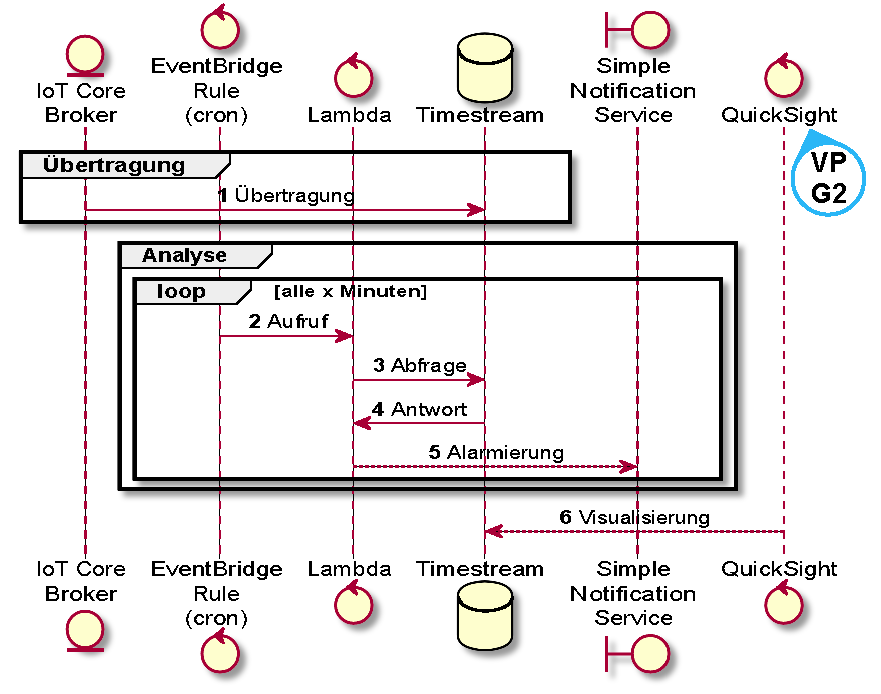
\includegraphics[width=\textwidth]{graphics/batch-ra.pdf}
\caption{Sequenzdiagramm Batch Verarbeitung}
\label{abb:SequenceBatchRA}
\end{figure}



\subsection{Verteilungssicht}
In der folgenden \autoref{abb:TopLevelDBRA} ist die Verteilungssicht der Referenzarchitektur gemeinsam mit den Variationspunkten gezeigt. Variationspunkte mit Präfix G können dabei auch auf bereits definierte Variationspunkte der Echtzeitreferenzarchitektur referenzieren.
\begin{figure}[H]
\centering
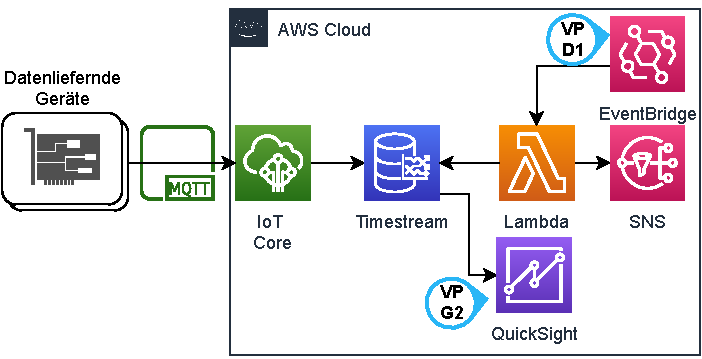
\includegraphics[width=\textwidth]{graphics/DB-RA-Overview.pdf}
\caption{Verteilungssicht}
\label{abb:TopLevelDBRA}
\end{figure}

\vp{D1}: EventBridge bietet den zeitlich geplanten Aufruf von Zielen wie Lambda an. Wenn keine kontinuierliche Überwachung gewünscht ist, kann die Lambda auch auf Bedarf ausgelöst werden. Dies wäre beispielsweise durch ein vorgelagertes API Gateway möglich. Über dieses muss dann der Zeitraum übergeben werden, für welchen die aktuelle Analyse durchgeführt werden soll.

\textbf{Variationspunkt G2:} Hier wird eine Dashboardinglösung, im speziellen der \ac{AWS} eigene Dienst QuickSight vorgesehen. Dies erfolgt, damit Benachrichtigungen, die via \ac{SNS} versendet werden, leicht für die Benachrichtigten nachvollziehbar sind. Wenn also beispielsweise eine Anomalie erkannt wurde, kann dies mit einer Visualisierung nachvollzogen werden, um dann entsprechend zu handeln. Wichtig ist, dass die Visualisierung sowohl von den Originaldaten aus dem Speicher von Timestream gespeist wird, als auch aus der Analyse. Das für und wieder des Einsatzes wurde auch bereits in \vpref{G2} der Echtzeitarchitektur diskutiert. Alternativ ist Timestream auch mit Grafana und damit dem Managed Service von Grafana integriert.\footcite[Vgl.][]{AmazonWebServicesInc..o.J.bm}\nzitat\footcite[Vgl.][]{Dutt.2020} Grafana kann dabei ebenfalls als Dashboardinglösung verwendet werden und kostet dabei das selbe wie die Standard Edition von QuickSight, nämlich 9\$ für Nutzende monatlich.\footcite[Vgl. auch im Foglenden][]{AmazonWebServicesInc..o.J.bn}\nzitat\footcite[Vgl.][]{AmazonWebServicesInc..o.J.bo} Erweiterte Kapazitäten bei QuickSight kosten 18\$ pro Monat für Nutzende. 




\subsection{Bausteinsicht}
In der folgenden \autoref{abb:ElementeDBRA} wird die Bausteinsicht als tiefere Dekomposition der Verteilungssicht, samt Variationspunkten dargestellt.
\begin{figure}[H]
\centering
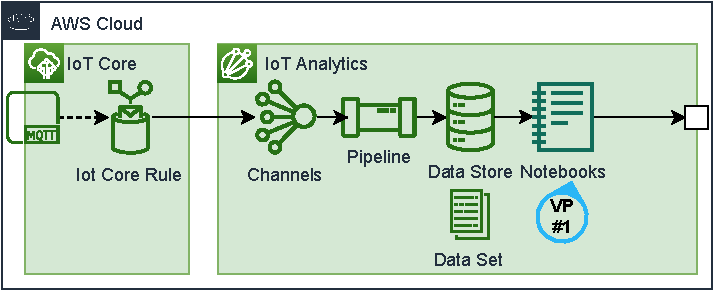
\includegraphics[width=\textwidth]{graphics/DB-RA-Elements.pdf}
\caption{Bausteinsicht}
\label{abb:ElementeDBRA}
\end{figure}

\vp{E1}: Timestream bietet aktuell zwei Speicherklassen an und hat eine Speicherklasse, die für die Zukunft angekündigt ist. Aktuell verfügbar sind \ac{RAM}-basierter Speicher, der teurer ist und magnetischer \ac{HDD}-Speicher, der günstiger ist. Mittels sogenannter \textit{retention policies} können Daten zwischen den Speicherklassen verschoben werden.\footcite[Vgl. auch im Folgenden][]{AmazonWebServicesInc..o.J.bp} Dabei können Daten vom \ac{RAM}-Speicher in den \ac{HDD}-Speicher verschoben werden und vom \ac{HDD}-Speicher gelöscht werden. Beim finalen Löschen der Daten sind die jeweiligen Anforderungen an Datenaufbewahrung der instanziierenden Architektur zu beachten. So können beispielsweise Langzeitanalysen notwendig sein, die auf einen Datenbestand von mehreren Monaten oder Jahren zugreifen müssen. Da Timestream aber auch nach Speicher abgerechnet wird, sind \textit{retention policies} sowohl von \ac{RAM} zu \ac{HDD} als auch zur Löschung von Inhalt vom \ac{HDD}-Speicher einzurichten. Zu beachten ist, dass die Gesamtaufbewahrungsdauer sich aus der Summe beider Aufbewahrungszeiten ergibt. Die Einstellung der \ac{RAM} zu \ac{HDD} retention policy ist abhängig von \vpref{E2} und \vpref{E5}, da je nach Abfragerhythmus und abgefragter Datenmenge für Analysen eine verlängerte Aufbewahrung im \ac{RAM} zur beschleunigten Analyse sinnvoll ist. Für die \ac{SQL}-Abfragen wird kein Unterschied zwischen Speicherart gemacht, bis auf die technisch bedingte höhere Ausführungsdauer auf \ac{HDD}-Speichern.

\vp{E2}: \ac{SQL}-Abfragen in Timestream sind auf mehrere Arten optimierbar. Zum einen wird die abgefragte Datenmenge in Rechnung gestellt, was eine präzise Einschränkung der Abfrage mit \mintinline[breaklines]{sql}{WHERE} Bedingungen und einem genauen \mintinline[breaklines]{sql}{SELECT} notwendig macht. Zusätzlich ist die Datenabfrage in zwei Modellen möglich: dem flachen Modell und dem Zeitreihenmodell. \footcite[Vgl. auch im Folgenden][]{AmazonWebServicesInc..o.J.bq} Das flache Modell schreibt, wie in \autoref{tab:flat-timestream} gezeigt, für jeden Messwert eine eigene Zeile. Entsprechend muss der Messwert in der \mintinline[breaklines]{sql}{WHERE} Bedingung spezifiziert werden.

\begin{table}[H]
\centering
\begin{tabular}{|l|l|l|l|l|}
\hline
time & \begin{tabular}[c]{@{}l@{}}Dimension A\\ (Sensorname)\end{tabular} & measure\_name & \begin{tabular}[c]{@{}l@{}}measure\_value\\ ::double\end{tabular} & \begin{tabular}[c]{@{}l@{}}measure\_value\\ ::bigint\end{tabular} \\ \hline
\begin{tabular}[c]{@{}l@{}}2021-05-10\\ 23:59:59\end{tabular} & sensora & co2 & null & 500 \\ \hline
\begin{tabular}[c]{@{}l@{}}2021-05-10\\ 23:59:59\end{tabular} & sensorb & temperature & 25.5 & null \\ \hline
\end{tabular}
\caption{Beispiel flaches Datenabrufmodell}
\label{tab:flat-timestream}
\end{table}

Gegensätzlich dazu gibt das Zeitreihenmodell, welches sich beispielsweise mit der \\ \mintinline[breaklines]{sql}{CREATE_TIME_SERIES} Funktion erzeugen lässt, \ac{JSON} Arrays zurück. Diese sehen wie folgt aus: \mintinline[breaklines]{json}{[{"time":"2021-05-10 23:59:59","value":500}]}. Timestream bietet für diese Zeitreihen spezielle Funktionen, wie beispielsweise die Interpolation fehlender Werte an.



\vp{E3}: Der Programmcode und die Laufzeit der Lambdafunktion in diesem Variationspunkt sind je nach Anforderungen und Kentnissen des Implementierungsteams bei der Instanziierung dieser Referenzarchitektur anzupassen/neu zu schreiben. In \anhangref{anhang:batch-codesample} ist beispielhaft eine Lambdafunktion, geschrieben in Javascript für die Node.js Laufzeitumgebung, gezeigt. Diese Lambdafunktion sendet eine \ac{SQL}-Abfrage zur Zählung von schwellwertüberschreitenden Werten einzelner Sensoren. Folgend werden die Ergebnisse ausgewertet und für jeden Sensor mit überschreitenden Messwerten eine Benachrichtigung via SNS und ein \textit{shutdown}-Befehl an den Sensor via \ac{MQTT} versendet. Zu beachten ist, dass Lambdafunktionen einen Timeout von 15 Minuten haben..\footcite[Vgl.][]{AmazonWebServicesInc..o.J.bv} Sollten besonders aufwändige Auswertungen durch die Lambdafunktion durchgeführt werden, sollte sie in ein Orchestrierungsdienst wie Step Functions eingebunden werden. Step Functions kann Aufgaben wie automatische Neuversuche oder Fortsetzung der Abfrage durch Übergabe der Abfrage-ID von Timestream erledigen.

\vp{E4}: Unabhängig von dem in \vpref{G2} gewählten Dienst ist es möglich, individuelle Dashboards mit unterschiedlichen Interaktionsmöglichkeiten zu erstellen. So können beispielsweise sogenannte \textit{drill-downs} den Nutzenden Entscheidungsträgern helfen, dynamisch die Datenbereiche anzupassen. Ein Dashboard in QuickSight kann beispielsweise wie folgt aussehen:
\begin{figure}[H]
\centering
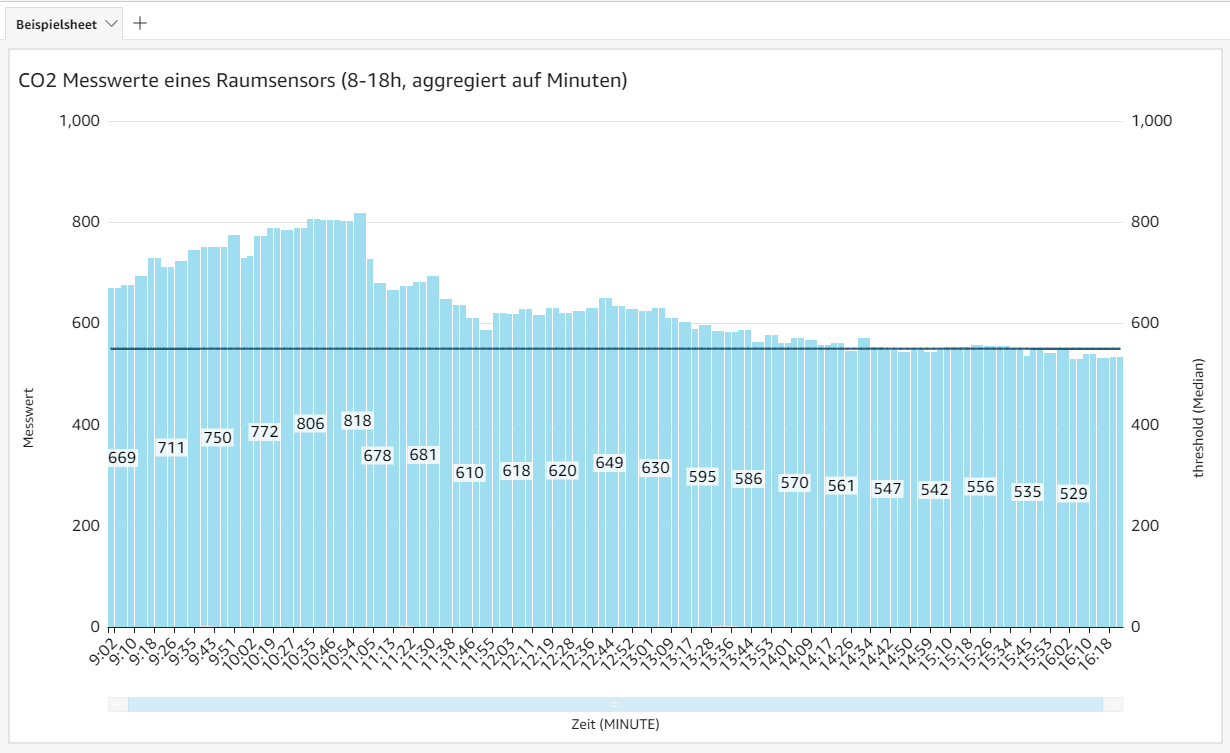
\includegraphics[width=\textwidth]{graphics/QuickSight-Beispiel.png}
\caption{Dashboard in QuickSight}
\label{abb:DashboardDBRA}
\end{figure}


\vp{E5}: EventBridge Regeln können unterschiedlich eingestellt werden. Abhängig von den Anforderungen der instanziierenden Architektur, kann entweder ein Aufruf alle x Minuten, Stunden oder Tage eingestellt werden, oder für mehr Anpassung eine Rate mittels einer abgewandelten, \textit{cron}-Syntax konfiguriert werden. Ein cron-Ausdruck, um die Regel alle 10 Minuten an Werktagen zwischen 9 und 17.00 Uhr auszulösen, sähe wie folgt aus: \mintinline[breaklines]{bash}{0/10 9-17 ? * MON-FRI *}. Der Ausdruck wird in \ac{UTC}-Zeit ausgeführt, was eine ein- oder zweistündige Verschiebung von der deutschen Zeit bedeutet.

\textbf{Variationspunkt G5}: Dieser Variationspunkt ist in der Bedeutung identisch zum \vpref{G5} der Echtzeitreferenzarchitektur.

\TodoW{Networking}

\subsection{Anforderungen}
Folgend wird für die Batch Architektur dargestellt, wie die einzelnen Anforderungen mittels der Referenzarchitektur addressierbar sind.
\subsubsection{Anwendbarkeit auf Monitoringdaten (IT)}
Timestream unterstüzt wie die Kinesis Familie diverse Zeitreihendaten. Es ist ebenfalls prinzipiell möglich Logdaten aufzubewahren, da der interne Datentyp \textit{varchar} Strings mit bis zu 2 GB Länge erlaubt.\footcite[Vgl.][]{AmazonWebServicesInc..o.J.br} Da aber große Datenmengen in einzelnen Variablen durch die doppelten Kosten für Speicherung und Abfrage sich weniger eignen als beispielsweise numerische Messwerte, sollte auf die Anwendung auf Logs verzichtet werden.

Die Nutzung zur Speicherung von Metriken hingegen ist explizit im Rahmen von \textit{DevOps}-Anwendungsfällen für Timestream vorgesehen.\footcite[Vgl.][]{AmazonWebServicesInc..o.J.ak}\nzitat\footcite[Vgl.][]{Das.2020} Ohne spezialisierte Applikation, die beispielsweise in Kinesis Data Analytics mit Flink Laufzeitumgebung laufen könnte und von Kinesis Data Firehose gespeist wird, ist es jedoch nicht möglich CloudWatch Metriken in Timestream zu laden.\footcite[Vgl.][]{Riddle.2021} Alternativ können Metriken wie von \citeauthor{Pochiraju.2020} vorgeschlagen, über \ac{MQTT} und \AWSIOT{} Core in Timestream eingespeist werden.\footcite[Vgl.][]{Pochiraju.2020} Das eine eigene Applikation verwendet werden muss, um Daten via Kinesis oder \ac{MQTT} einzuspeisen, wertet die Tauglichkeit für Monitoring-Usecases gegenüber der Echtzeitarchitektur ab.


\subsubsection{Anwendbarkeit auf Sensordaten (IoT)}
Durch die native Integration mit \AWSIOT{} Core ist eine Integration mit Datensätzen von Sensoren, die via \ac{MQTT} übermittelt wurden vollständig verwaltet möglich. Metadaten der Sensoren können zur Attributierung bei der Auswertung mittels der Dimensionen übermittelt werden, Messwerte als eben solche. Die Menge an Erkenntnissen, die sich aus der Analyse der Sensordaten in Timestream gewinnen lassen, ist wesentlich von \vpref{E5} und damit der Analysefrequenz abhängig.

\subsubsection{Handling von Events, Messwerten und \enquote{Streaming}}
Timestream ist vollständig verwaltet und es sind keine Infrastrukturkomponenten zur Skalierung anzupassen. Da laut Aussage von \ac{AWS} mit dem Dienst Billionen Datenpunkte pro Tag nahe der Echtzeit verarbeitet und abgefragt werden können, ist zu erwarten, dass auch hochfrequente Datenreihen in angemessener Zeit gespeichert werden können.\footcite[Vgl.][]{AmazonWebServicesInc..2020g} Dabei wäre es, wenn die Dateneingangslogik selbst zu schreiben wäre möglich, dass wiederholbare Fehler auftreten. Da aber die Daten automatisiert nach dem Eingang im \ac{MQTT} Broker \AWSIOT{} Core in Timestream gespeichert werden, ist dies nicht nötig. Ein mögliches Problem gibt es maximal bei der Überttragungslatenz zwischen \AWSIOT{} Core und Timestream, auf die kein Einfluss genommen werden kann.
Da Timestream abseits der numerischen Datentypen auch Datentypen vie \textit{varchar} anbietet, ist es möglich auch Events in Timestream abzuspeichern.\footcite[Vgl.][]{AmazonWebServicesInc..o.J.r}


\subsubsection{Automatisierte operative Entscheidungen}
Das Codebeispiel in \anhangref{anhang:batch-codesample} demonstriert, dass es möglich ist, basierend auf den Ergebnissen einer Abfrage automatisiert Abfragen durchzuführen. Dabei zu beachten ist jedoch, dass durch die Intervallverzögerung Aktionen im schlechtesten Fall nach genau $t$ Minuten, nach dem Ereignis ausgelöst werden. Dabei ist $t$ das Intervall zwischen einzelnen Ausführungen, wie beschrieben in \vpref{E5}. Dies kann bei kritischen Aktionen, die möglichst schnell ausgeführt werden sollen jedoch die akzeptable Raktionszeit stark überschreiten. Sollte Timestream ähnlich zu Amazons DynamoDB integrierte Streams als Feature bekommen, welche Änderungen am Datensatz zur Verarbeitung an Plattformen wie Lambda senden, wäre dieses Problem addressierbar.

\subsection{Produktives Monitoringkonzept}
In \autoref{tab:cloudwatch-metrics-db} sind die zu überwachenden Cloud-Watch Metriken der in der Referenzarchitektur verwendeten Dienste gezeigt. Dies umfasst TimeStream, Lambda, \ac{SNS}, \AWSIOT{} Core und EventBridge.\footcite[Vgl.][]{AmazonWebServicesInc..o.J.be}\nzitat\footcite[Vgl.][]{AmazonWebServicesInc..o.J.bf}\nzitat\footcite[Vgl.][]{AmazonWebServicesInc..o.J.bc}\nzitat\footcite[Vgl.][]{AmazonWebServicesInc..o.J.az}\nzitat\footcite[Vgl.][]{AmazonWebServicesInc..o.J.bl}


\begin{table}[H]
\centering
\begin{tabular}{|l|l|l|l|}
\hline
Dienst & Metrik & Ursache & Detektionsart \\ \hline
\rowcolor[HTML]{F5F5F5} 
\ac{SNS} & NumberOfNotificationsFailed & Dienstfehler & Schwellwert \\ \hline

\multirow{2}{*}{\AWSIOT{} Core} & RuleMessageThrottled & \begin{tabular}[c]{@{}l@{}}Dienstfehler/\\ Benutzungsfehler\end{tabular} & Schwellwert \\ \cline{2-4} 
 & Failure & \begin{tabular}[c]{@{}l@{}}Dienstfehler/\\ Benutzungsfehler\end{tabular} & Schwellwert \\ \hline
 
\rowcolor[HTML]{F5F5F5} 
\cellcolor[HTML]{F5F5F5} & SystemErrors & Dienstfehler & Schwellwert \\ \cline{2-4} 
\rowcolor[HTML]{F5F5F5} 
\cellcolor[HTML]{F5F5F5} & UserErrors & Benutzungsfehler & Schwellwert \\ \cline{2-4} 
\rowcolor[HTML]{F5F5F5} 
\multirow{-3}{*}{\cellcolor[HTML]{F5F5F5}TimeStream} & SuccessfulRequestLatency & \begin{tabular}[c]{@{}l@{}}Dienstfehler/\\ Benutzungsfehler\end{tabular} & Anomalie \\ \hline

\multirow{3}{*}{Lambda} & Duration & \begin{tabular}[c]{@{}l@{}}Dienstfehler/\\ Benutzungsfehler\end{tabular} & Anomalie \\ \cline{2-4} 
 & Errors & \begin{tabular}[c]{@{}l@{}}Dienstfehler/\\ Benutzungsfehler\end{tabular} & Schwellwert \\ \cline{2-4} 
 & Throttles & Benutzungsfehler & Schwellwert \\ \hline
 
\rowcolor[HTML]{F5F5F5} 
\cellcolor[HTML]{F5F5F5} & FailedInvocations & Dienstfehler & Anomalie \\ \cline{2-4} 
\rowcolor[HTML]{F5F5F5} 
\multirow{-2}{*}{EventBridge} & ThrottledRules & Dienstfehler & Schwellwert \\ \hline
\end{tabular}
\caption{CloudWatch Metriken}
\label{tab:cloudwatch-metrics-db}
\end{table}

\AWSIOT{} Core, \ac{SNS} und Timestream übermittelt Metriken in einminütiger Auflösung.\footcite[Vgl.][]{AmazonWebServicesInc..o.J.az}\nzitat\footcite[Vgl.][]{AmazonWebServicesInc..2021b}\nzitat\footcite[Vgl.][]{AmazonWebServicesInc..o.J.be} 
Bei Lambda können die übermittelten Metriken bis nach Ende einer Ausführung übermittelt werden, weshalb die Auflösung der Metriken unpräzise sein kann. Insgesamt lässt sich aufgrund der teilweise verketteten Metriken leicht erkennen, wenn kaskadierende Fehler auftreten. So sind beispielsweise \textit{FailedInvocations} von EventBridge ein Hinweis darauf, dass es Probleme bei der Ausführung von Lambda Funktionen gab.



\subsection{Know-how für instanziierende Architekturen}
Während Timestream zum Start 2020 allein in Irland (eu-west-1) für die EU verfügbar war, ist Timestream für die Region eu-central-1 (Frankfurt) mittlerweile verfügbar.\footcite[Vgl.][]{AmazonWebServicesInc..2020g}\nzitat\footcite[Vgl.][]{AmazonWebServicesInc..o.J.q} Dies erleichtert die Integration in bestehende Dienste, die bereits in Frankfurt provisioniert wurden.

Zeitreihen mit Messwerten und Metadaten werden innerhalb von Timestream als Dimensionen oder Messwerte hinterlegt. Dimensionen und Messwerte haben jeweils einen Namen und einen Wert. Dabei sind als Dimensionen alle Metadaten des übermittelnden Sensors oder der übermittelnden Applikation denkbar. Beispiele für solche Dimensionen wären Name oder Standort, während Messwerte beispielsweise \coo{} Messungen, Temperaturen, CPU Auslastung oder \ac{RAM}-Verbrauch sein können. Timestream rechnet pro Schreibzugriff die Summe aller Namen von Dimensionen und Messwerten und deren Werte (inklusive der Zeitdimension mit aktuellem Zeitstempel) als Speicherplatz ab.\footcite[Vgl. auch im Folgenden][]{AmazonWebServicesInc..o.J.bs} Bei gruppierten Schreibzugriffen können gemeinsame Attribute und Werte zusammengefasst werden, um die Anzahl an Schreibzugriffen zu vermindern.
Aus der Unterteilung in Messwerte und Dimensionen ergeben sich auch Optimierungen der Datenmodellierung. So gibt es beispielsweise die Möglichkeit, derivative Werte, sofern sie eine niedrige Kardinalität besitzen als Dimensionen statt als Messwerte zu speichern.\footcite[Vgl. auch im Folgenden][]{AmazonWebServicesInc..o.J.bt} Dies bringt aber den Nachteil mit sich, dass entsprechend drei verschiedene Zeitreihen entstehen würden, was bei der Abfrage zu beachten ist. Da Dimensionsnamen ebenfalls Speicherplatz verbrauchen, sind die Namen entsprechend des Ockhams Rasiermesser zu gestalten und die einfachste und kürzeste Variante auszuwählen. Bei der Datenmodellierung ist auch zu beachten, dass Messwerte entsprechend ihres eigentlichen Datentyps gespeichert werden und keine unbeabsichtigte Konversion in z.B. das \textit{varchar} Format auftritt. Da Messwerte bei Erstanlage eines Messwertes in einer Tabelle fest mit einem Datentypen assoziiert werden, ist eine Neuanlage mit entsprechender Datenmigration notwendig um Fehler zu korrigieren.





\section{Einsatzszenarien der Referenzarchitekturen}
Ob die Referenzarchitekturen im Tagesgeschäft eingesetzt werden können, soll anhand der Qualitätskriterien für Referenzarchitekturen überprüft werden. Aus diesem Grund wurden in  \anhangref{anhang:interview-philipp-03.05.2021}, \anhangref{anhang:interview-viet-04.05.2021} und \anhangref{anhang:interview-jan-04.05.2021} Interviews mit diversen Stakeholdern der Cloud Entwicklung geführt. Dabei war eine Verständlichkeit trotz der unterschiedlichen technischen Hintergründe der Interviewpartner zu erkennen. Ebenfalls haben die Stakeholder die Referenzarchitekturen akzeptiert und sahen die Qualität als zufriedenstellend an. Aufgrund des Feedbacks aus \anhangref{anhang:interview-viet-04.05.2021} wurden zwischen dem Stand zur Zeit des Interviews und dem finalen Stand Diagramme in mehrere aufgeteilt. Dies dient auch der Behebung des Zuordnungsproblems aus \anhangref{anhang:interview-jan-04.05.2021}.

Eine Zugänglichkeit und ein Zugriff durch die Mehrheit der Organisation ist auf zweierlei Arten sichergestellt: Zum einen wird die fertige Bachelorarbeit an mehreren Stellen in den internen Wissensmanagementsystemen wie Confluence publiziert und zum anderen ist die Bachelorarbeit auf GitHub open source verfügbar.\footnote{Siehe \url{https://github.com/LukvonStrom/Bachelorarbeit}} Eine Wartbarkeit ist durch den offenen Prozess des Forkens via dem Versionsverwaltungstool Git und der offenen MIT-Lizenz, wie auch in \anhangref{anhang:interview-philipp-03.05.2021} erläutert, gewährt. Die Hauptprobleme dieser Domäne sind insofern adressiert, dass die Referenzarchitekturen mit den $\kappa$ und \ac{OLAP} Patterns auf etablierten Mustern basieren. Wertschöpfung für den Betrieb ist insofern garantiert, dass der Bedarf der Behandlung des Themas aus dem Geschäftsalltag entstanden ist, wie in \anhangref{anhang:interview-philipp-03.05.2021} erläutert.


Im Folgenden soll beleuchtet werden, wofür sich welche der beiden entwickelten Referenzarchitekturen besser eignet.
Für das Monitoring eignet sich die in \autoref{chap:ra-rt} beschriebene Referenzarchitektur besser, da eine enge Integration sowohl mit CloudWatch Metrics als auch CloudWatch Logs besteht. So lassen sich Analysen zu in der \ac{AWS}-Cloud laufenden Workloads einfach durchführen. Dadurch, dass keine eigene Software geschrieben werden muss, um die Metriken in das Analysesystem zu laden, ist dieser Usecases wesentlich günstiger im Sinne des firmenseitigen Investments abgedeckt.

Beide Referenzarchitekturen integrieren sich gut mit \AWSIOT{} Core und besitzen damit eine wichtige Voraussetzung zur Analyse der \ac{IoT} Daten. Gemäß der in \autoref{chap:datenwert} erläuterten Datenhalbwertszeit ist eine Auswahlentscheidung auch in Abhängigkeit von den Analyseanforderungen der Share- und Stakeholder der instanziierenden Architektur zu treffen. Unter Einsatz einer Dashboardinglösung wie QuickSight oder Grafana können historische Daten bei beiden Referenzarchitekturen auch Entscheidern zugänglich gemacht werden, wenn die Datenablage in \ac{S3} erfolgt. 

Sollten längere Aufbewahrungsfristen der Daten über 30 Tage hinaus gewünscht sein, ist die Batch Architektur zu empfehlen, da die Datenhaltung großer Mengen an historischen Daten zu Analysezwecken möglich ist. Alternativ könnten beide Architekturen auch, ähnlich zur $\lambda$-Architektur kombiniert werden, um Timestream als Aufbewahrungslösung für ältere Daten bei Bedarf zu verwenden und Analysen über Echtzeitdaten mittels Kinesis durchzuführen. Bei einer solchen Kombination wäre zu beachten, die Speicherklasse \ac{HDD} zu verwenden, da die Latenz von Abfragen dann weniger kritisch ist. Wenn eine intervallbasierte Auswertung tolerierbar ist, ist Timestream zu verwenden, da die Gesamtkosten abhängig von der Art der Abfragen und die Komplexität der Architektur niedriger sind, als bei der Echtzeitreferenzarchitektur.


Da die Referenzarchitekturen als verteilte Systeme mit mehreren Diensten diverse Fehlerquellen haben können, die sich dann symptomatisch in den gezeigten Metriken bemerkbar machen, sind genaue Tests zum Verständnis der Fehlerzustände wichtig. Im Rahmen des \textit{Chaos Engineerings} lassen sich gezielt Fehler in das System einführen um die Resilienz gegenüber diversester Fehlerquellen zu testen.\footcite[Vgl.][]{Augsten.2020} Bei den vorgestellten Referenzarchitekturen ist es zu empfehlen, regelmäßige Chaos Experimente durchzuführen um gezielt Fehlerszenarien wie doppelte Nachrichten, hohe Latenzen zwischen Diensten oder die temporäre Nichtverfügbarkeit einzelner Dienste zu simulieren und gezielt den Einfluss messen zu können. Folgend können Erkentnisse für den besseren Betrieb einer resilienten Dateninfrastruktur abgeleitet und dokumentiert werden. Für \ac{AWS} gibt es den Dienst Fault Injection Simulator, welcher Fehler in Schnittstellen zwischen Diensten erzeugen kann und gezielt auch einzelne Infrastrukturkomponenten beeinträchtigen kann.\footcite[Vgl.][]{Barr.2021b} Unter Verwendung dieses Dienstes ist es möglich, die beschriebenen Chaos Experimente durchzuführen.

In den vorliegenden Referenzarchitekturen wurde gemäß \autoref{abb:DimensionenUebersicht} eine \enquote{so tief wie notwendige} Dekomposition erreicht, indem Variationspunkte mit starken Auswirkungen in stärkerer Detailtiefe erklärt werden, während beide Referenzarchitekturen auf den selben Dekompositionssichten aufbauen.

Eine hohe Anwendbarkeit wurde von den diversen Stakeholdern wie oben beschrieben in \anhangref{anhang:interview-philipp-03.05.2021}, \anhangref{anhang:interview-viet-04.05.2021} und \anhangref{anhang:interview-jan-04.05.2021} attestiert.
In Sachen Allgemeingültigkeit wurde insofern ein leicht abgesenkter Standard erreicht, da sich aufgrund der Prioritäten des Dienstvergleiches, die durch wichtige Stakeholder durchgeführt wurden eine für die Zielorganisation spezifische Architektur ergeben hat. Andere Organisationen, die beispielsweise eine Übertragbarkeit zwischen Clouds als wichtiger empfinden, hätten möglicherweise alternative Dienste wie OpenSearch in der Batchverarbeitung gewählt, aufgrund eines anders priorisierten Vergleiches.